\chapter{Аналитический раздел}
\label{cha:analysis}

Известные на данный момент методы распознавания жестовых символов, как правило, реализуют три этапа обработки информации:

\begin{enumerate}
	\item получение данных о жесте;
	\item предобработка данных;
	\item классификация жестов.
\end{enumerate}

В качестве входных данных можно использовать кинематические трехмерные модели рук, получаемых с помощью специальных устройств ввода, таких как Microsoft Kinect\cite{Wang} и Leap Motion Controller\cite{Mohandes}. Такие методы обеспечивают достаточно высокую точность распознавания, позволяя обнаруживать различные жесты, но при этом требуют большого объема вычислений и наличия обширной базы данных, содержащей все жесты. Также данные методы получения информации о жесте требуют наличия дополнительных устройств ввода. Из-за этого, данную группу способов получения информации о жестах решено не рассматривать в данной работе.

В качестве другого источника данных можно использовать RGB изображения, полученные, например, с web-камеры ПК или камеры смартфона. Преимуществом данного подхода является распространенность данных устройств ввода. Web-камерой в наше время оснащен каждый ноутбук, а смартфонами владеет 45\% населения Земли \cite{smartfones}.

\section{Алгоритмы предобработки изображения кисти руки, применимых к распознаванию жестовых символов}

Скорость и качество работы алгоритмов классификации во многом зависит от исходных данных. Например, для классификации жестов с помощью скрытой марковской модели\cite{Zhang} основные признаки получаются из изображения рук в разноцветных перчатках. Тем самым, важно подобрать метод предобработки изображения таким образом, чтобы его применение в итоговом методе упрощало процесс классификации, не увеличивая при этом общее время работы. Известные алгоритмы, применимые для достижения данной цели, можно разделить на следующие группы:

\begin{itemize}
	\item выделение контура фигуры;
	\item выделение силуэта кисти руки;
	\item построение скелета кисти руки.
\end{itemize}

Рассмотрим каждую из этих групп.

\subsection{Выделение контура фигуры}

Для выделения контура кисти руки можно использовать детекторы границ, определяющие градиент яркости черно-белого изображения. Поэтому предварительным этапом данных методов является преобразование изображения из цветного в черно-белое. К вышеуказанным методам относят:

\begin{itemize}
	\item оператор Собеля\cite{Sobel};
	\item оператор Прюитт\cite{Prewitt};
	\item перекрестный оператор Робертса\cite{Roberts};
	\item оператор Кэнни\cite{Canny}.
\end{itemize}

\section*{Операторы Собеля, Прюитт и Робертса}

Принцип работы данных алгоритмов \cite{Sobel,Prewitt,Roberts} заключается в свертке изображения двумя сепарабельными целочисленными фильтрами. Общая схема работы методов представлена на рис. \ref{an:sobel}.

\begin{figure}[!h]
	\centering
	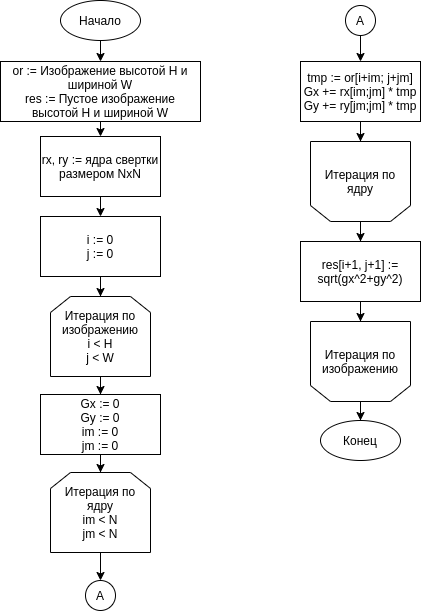
\includegraphics[width=0.6\textwidth]{inc/img/sobel_block}
	\caption{Общая схема алгоритмов определения границ изображения}
	\label{an:sobel}
\end{figure}

Разница алгоритмов заключается в способе задания ядер свертки:

Оператор Собеля:

\begin{eqnarray}\label{eq:sobel-matrixs}
G_x = \begin{bmatrix}
-1 & 0 & 1\\
-2 & 0 & 2\\
-1 & 0 & 1\\
\end{bmatrix} 
G_y = \begin{bmatrix}
-1 & -2 & -1\\
0 & 0 & 0\\
1 & 2 & 1\\
\end{bmatrix}
\end{eqnarray}

Оператор Прюитт:

\begin{eqnarray}\label{eq:prewitt-matrixs}
G_x = \begin{bmatrix}
-1 & 0 & 1\\
-1 & 0 & 1\\
-1 & 0 & 1\\
\end{bmatrix} 
G_y = \begin{bmatrix}
-1 & -1 & -1\\
0 & 0 & 0\\
1 & 1 & 1\\
\end{bmatrix}
\end{eqnarray}

Из-за меньшего значения средних элементов итоговое изображение имеет более явный эффект сглаживания.

Перекрестный оператор Робертса:

\begin{eqnarray}\label{eq:roberts-matrixs}
G_x = \begin{bmatrix}
1 & 0\\
0 & -1
\end{bmatrix} 
G_y = \begin{bmatrix}
0 & 1\\
-1 & 0
\end{bmatrix}
\end{eqnarray}

Недостатком данного метода является отсутствие четко выраженного центрального элемента у ядра свертки. Но эта особенность алгоритма обуславливает высокую скорость обработки изображения.

В итоговом изображении в каждый пиксель записывается значение изменения яркости пикселя исходного изображения относительно соседних, вычисляемое по формуле $G=\sqrt{G_x^2+G_y^2}$, т. е. чем выше итоговое число, тем вероятнее, что данный пиксель находится на границе.

\section*{Оператор Кэнни}

Метод\cite{Canny} был разработан с целью удовлетворения следующим условиям:

\begin{itemize}
	\item хорошее обнаружение (Кэнни трактовал это свойство как повышение отношения сигнал/шум);
	\item хорошая локализация (правильное определение положения границы);
	\item единственный отклик на одну границу.
\end{itemize}

Схема работы алгоритма представлена на рис. \ref{an:canny}. Рассмотрим каждый этап подробнее с наглядной визуализацией обработки. Для этого применим данный оператор шаг за шагом к изображению, приведенному на рис. \ref{fig:canny}a.

\begin{figure}[!h]
	\centering
	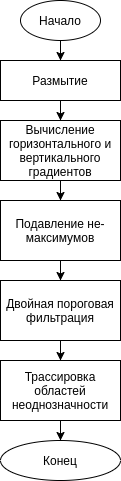
\includegraphics[width=0.15\textwidth]{inc/img/canny-block}
	\caption{Схема алгоритма оператора Кэнни}
	\label{an:canny}
\end{figure}

\begin{figure}[ht!]
	\begin{minipage}[h]{0.49\linewidth}
		\center{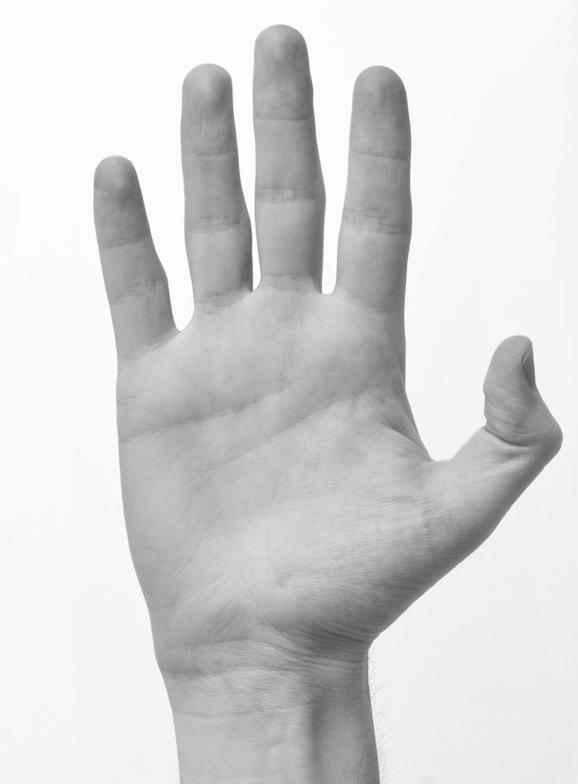
\includegraphics[width=0.5\linewidth]{inc/img/bmstu_gray} \\ а)}
	\end{minipage}
	\hfill
	\begin{minipage}[h]{0.49\linewidth}
		\center{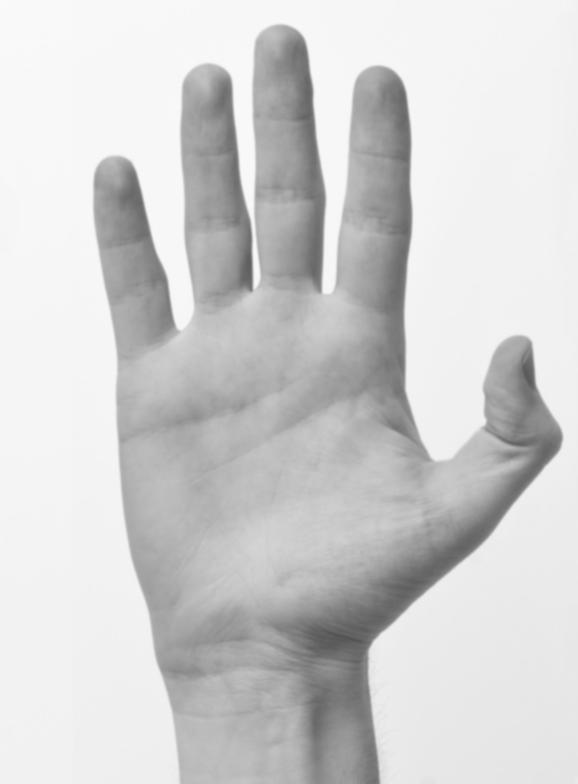
\includegraphics[width=0.5\linewidth]{inc/img/bmstu_smoothed} \\ б)}
	\end{minipage}
	\begin{minipage}[h]{0.49\linewidth}
		\center{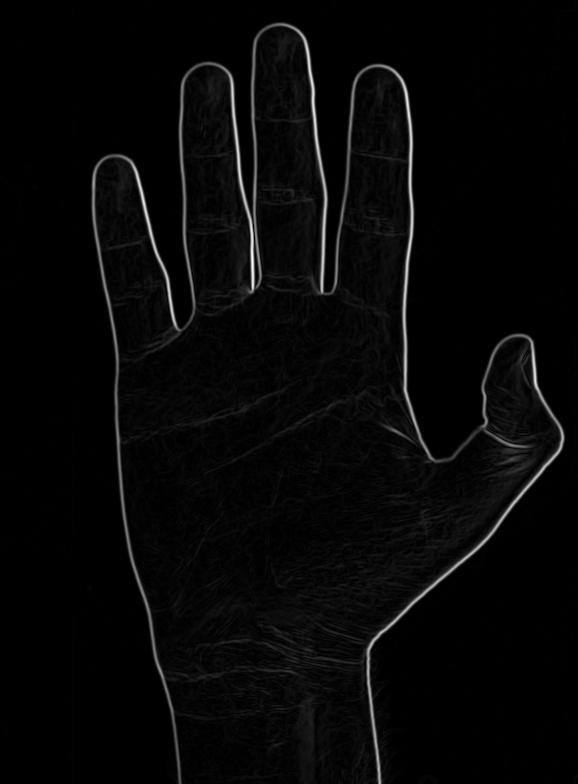
\includegraphics[width=0.5\linewidth]{inc/img/bmstu_gradient} \\ в)}
	\end{minipage}
	\hfill
	\begin{minipage}[h]{0.49\linewidth}
		\center{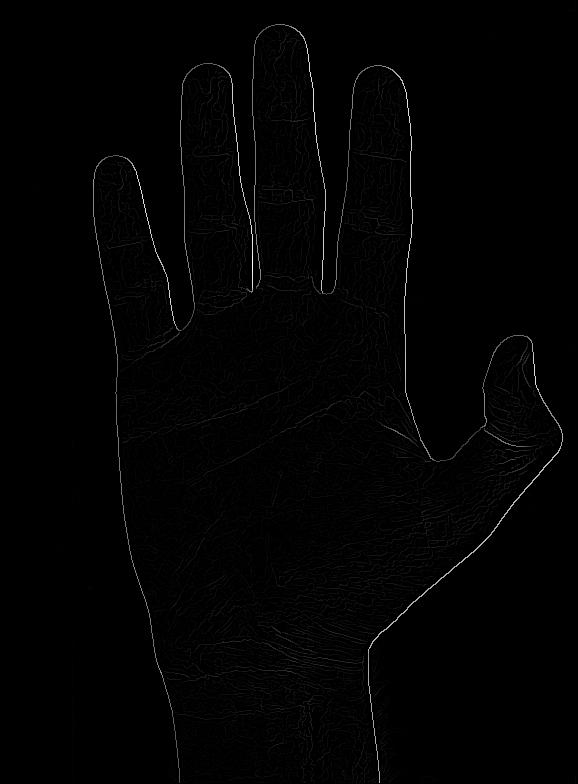
\includegraphics[width=0.5\linewidth]{inc/img/bmstu_non_max} \\ г)}
	\end{minipage}
	\begin{minipage}[h]{0.49\linewidth}
		\center{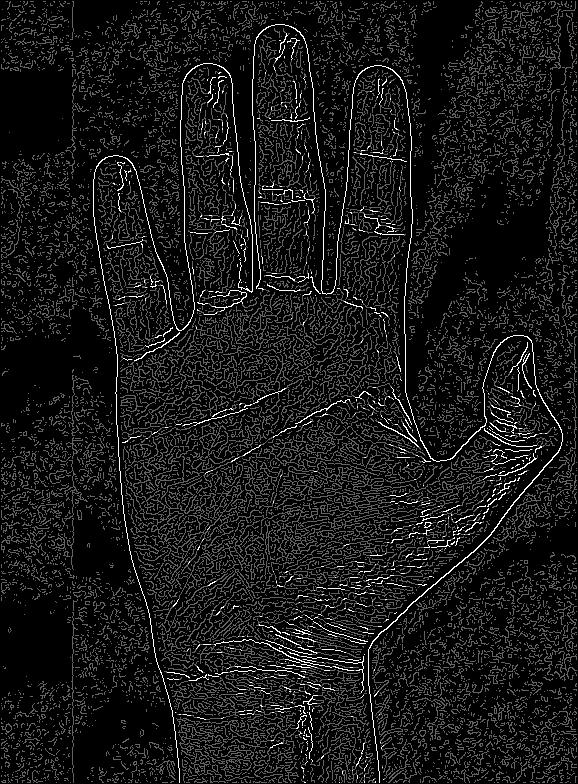
\includegraphics[width=0.5\linewidth]{inc/img/bmstu_threshold} \\ д)}
	\end{minipage}
	\hfill
	\begin{minipage}[h]{0.49\linewidth}
		\center{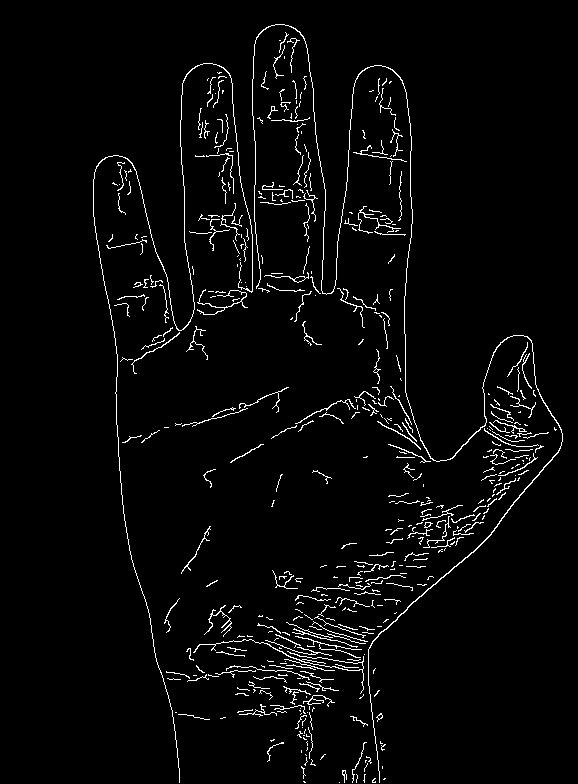
\includegraphics[width=0.5\linewidth]{inc/img/bmstu_final} \\ е)}
	\end{minipage}
	\caption{Результаты экспериментального исследования этапов оператора Кэнни: а) исходное изображение; б) применение размытия; в) поиск градиентов; г) подавление	не-максимумов; д) двойная пороговая фильтрация; е) трассировка областей неоднозначности}
	\label{fig:canny}
\end{figure}

\begin{enumerate}
	\item Размытие изображения. Данный этап, как видно на рис. \ref{fig:canny}б, необходим для устранения лишних шумов, способных понизить качество последующих	этапов выделения границ.
	\item Поиск градиентов яркости. На данном этапе был применен оператор Собеля, описанный ранее. В результате на рис. \ref{fig:canny}в были получены точки, наиболее вероятно находящиеся на границах изображения\cite{Suharjito}.
	\item Подавление <<не-максимумов>>. Как видно на рис. \ref{fig:canny}г, на данном этапе отбрасываются точки, значение градиента которых не является локальным максимумом, т. е. такие точки являются ложными границами.
	\item Определение потенциальных границ с помощью двойной пороговой фильтрации. При этом используется два порога фильтрации:
	\begin{itemize}
		\item Все пиксели со значением больше верхней границы принимают максимальное значение (достоверная граница).
		\item Все пиксели со значением меньше нижней границы подавляются.
		\item Все пиксели со значением в диапазоне границ принимают фиксированное среднее значение. Их уточнение происходит на следующем этапе.
	\end{itemize}
	На рис. \ref{fig:canny}д представлен результат применения данной фильтрации с порогами 0.03 и 0.07. В результирующую достоверную границу была добавлена часть контура тени кисти.
	\item Трассировка области неоднозначности. После данного этапа, как видно на рис. \ref{fig:canny}е были отброшены все неопределенные границы, потому что они не были связаны с уже определенной границей.
\end{enumerate}

\subsection{Выделение силуэта кисти руки}
\label{cha:syl}
Помимо классических методов определения границ, можно использовать сегментацию по цвету кожи\cite{Phung}. Данный метод преобразует RGB изображение в бинарное с помощью фильтрации пикселей по цвету, близкому к цвету кожи. Для улучшения работы алгоритма перед фильтрацией изображение переводят в цветовое пространство YCrCb, в котором различные цвета кожи расположены близко друг к другу\cite{Siddharth}. Пример работы данного алгоримта представлен на рисунке \ref{anal:preproc}.

\begin{figure}[ht!]
	\begin{minipage}[h]{0.49\linewidth}
		\center{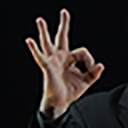
\includegraphics[width=0.5\linewidth]{inc/img/preprocessing/good_orig} \\ а)}
	\end{minipage}
	\hfill
	\begin{minipage}[h]{0.49\linewidth}
		\center{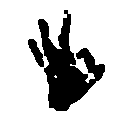
\includegraphics[width=0.5\linewidth]{inc/img/preprocessing/good_res} \\ б)}
	\end{minipage}
	\caption{Результат выделения кисти руки: а) исходное изображение; б) предобработанное изображение}
	\label{anal:preproc}
\end{figure}

Как правило, после бинаризации на изображении присутствуют шумы и артефакты, вызванные тем, что на фоновой части изображения находились пиксели,
попадающие в ограничения фильтра. Для их устранения можно использовать морфологические операции: «наращивание» и «эрозия»\cite{DIP}.

Пусть имеется бинарное изображение A и структурный элемент B c началом координат в его центре (рис. \ref{an:morph}).

\begin{figure}[!h]
	\centering
	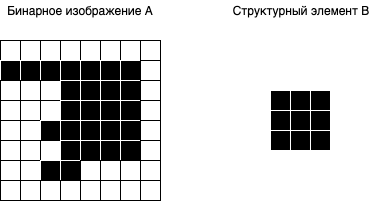
\includegraphics[width=0.6\textwidth]{inc/img/morf}
	\caption{Бинарное изображение и структурный элемент}
	\label{an:morph}
\end{figure}

Наращивание. Каждый раз, когда начало координат структурного элемента совмещается с единичным бинарным пикселем, ко всему структурному элементу применяется перенос и последующее логическое сложение с соответствующими пикселями бинарного изображения (рис. \ref{an:dil}).

\begin{figure}[!h]
	\centering
	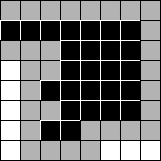
\includegraphics[width=0.3\textwidth]{inc/img/dil}
	\caption{Наращивание бинарного изображения A структурным элементом B}
	\label{an:dil}
\end{figure}

Эрозия. Если в некоторой позиции каждый единичный пиксель структурного элемента совпадает с единичным пикселем бинарного изображения, то выполняется логическое сложение центрального пикселя структурного элемента с соответствующим пикселем выходного изображения (рис. \ref{an:eros}).

\begin{figure}[!h]
	\centering
	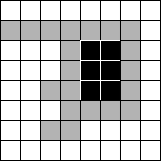
\includegraphics[width=0.3\textwidth]{inc/img/eros}
	\caption{Эрозия бинарного изображения A структурным элементом B}
	\label{an:eros}
\end{figure}

\subsection{Построение скелета кисти руки}

Для ускорения процесса классификации жеста руки можно использовать скелетную модель. Данный тип входных данных в силу своей специфики может упростить вычисление признаков, необходимых классификатору.

Для построения скелета кисти можно использовать метод построения скелета выпуклой фигуры\cite{DIP}.

В качестве выпуклой фигуры можно использовать результат работы метода выделения силуэта кисти руки, описанного в разделе \ref{cha:syl}.

В данном методе предлагается последовательное применение морфологической операции «эрозия» (рис. \ref{an:eros}) до тех пор, пока результатом следующей итерации не станет пустое изображение.

Недостатком данного метода являются побочные ветви скелета, образованные из-за возможной зашумленности или неточности фигуры. Другим недостатком можно считать высокую вероятность получения несвязного набора пикселей для всего скелета или обеспечения одинаковой ширины ветвей во всем скелете.

Для решения данных проблем можно обратиться к технологиям машинного обучения. Скелет кисти можно построить на основании ключевых точек, получаемых с помощью нейронной сети\cite{DNN}. Данная нейронная сеть определяет на изображении 22 ключевые точки, 21 из которых относится к кисти руки, а 22 — отмечают фон. Пример расположения точек представлен на рис. \ref{an:handpose}.

\begin{figure}[!h]
	\centering
	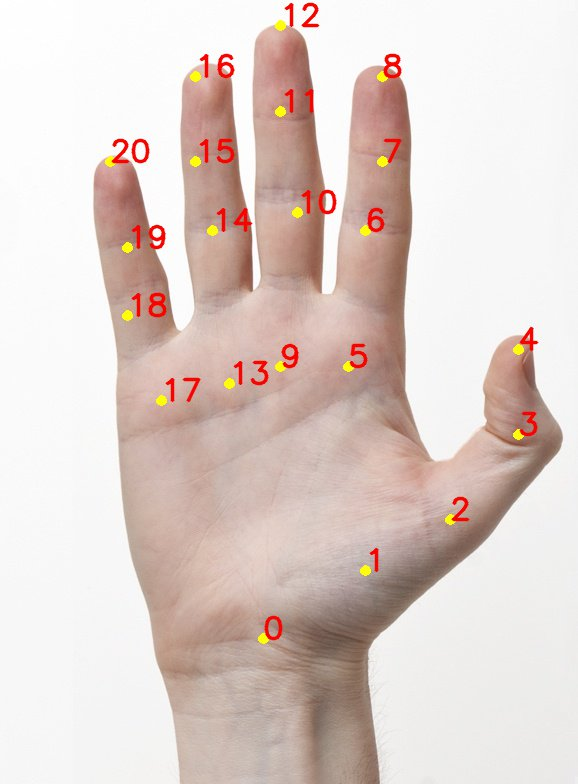
\includegraphics[width=0.3\textwidth]{inc/img/handpose-demo-keypoints}
	\caption{Ключевые точки кисти руки}
	\label{an:handpose}
\end{figure}

Далее для построения скелета необходимо соединить полученные точки в последовательностях, описанной в табл. \ref{an:poses-table}.

\begin{table}[h]
	\caption{\label{an:poses-table}Последовательность соединения ключевых точек}
	\begin{center}
		\begin{tabular}{|p{0.45\textwidth}|p{0.45\textwidth}|}
			\hline
			Ветвь скелета & Последовательность точек \\
			\hline
			Большой палец & 0$\rightarrow$1$\rightarrow$2$\rightarrow$3$\rightarrow$4 \\	
			\hline
			Указательный палец & 0$\rightarrow$5$\rightarrow$6$\rightarrow$7$\rightarrow$8\\	
			\hline
			Средний палец & 0$\rightarrow$9$\rightarrow$10$\rightarrow$11$\rightarrow$12 \\
			\hline
			Безымянный палец & 0$\rightarrow$13$\rightarrow$14$\rightarrow$15$\rightarrow$16 \\
			\hline
			Мизинец & 0$\rightarrow$17$\rightarrow$18$\rightarrow$19$\rightarrow$20 \\
			\hline
		\end{tabular}
	\end{center}
\end{table}

\subsection{Сравнение алгоритмов предобработки изображений}

Сравнительный анализ описанных выше методов был проведен в работе \cite{Tantsevov}. Каждый из алгоритмов был применен для обработки одинакового набора данных, состоящего из растровых изображений кистей рук; тестовая выборка составлялась из наборов данных, различающихся форматами изображений, их размерами и физиологическими особенностями кистей рук. Все данные находятся в открытом доступе:

\begin{itemize}
	\item ASL Alphabet. Image data set for alphabets in the American Sign Language;
	\item Hand Gesture of the Colombian sign language. Hand gestures, recognizing the numbers from 0 to 5 and the vowels;
	\item ASL Fingerspelling Images (RGB \& Depth);
	\item <<sign language between 0 9>>.
\end{itemize}

Замеры времени обработки каждого изображения для получения статистики проводились по минимальному, максимальному и среднему времени работы алгоритма. Результаты экспериментов представлены для каждого набора данных: для ASL Alphabet представлены в табл. \ref{tab:asl-alphaber}; для Hand Gesture of the Colombian sign language -- в табл. \ref{tab:colombian-alphaber}; для ASL Fingerspelling Images — в табл. \ref{tab:asl2-alphaber}; для <<sign language between 0 9>> — в табл. \ref{tab:datamix-alphaber}.

\begin{table}[h]
	\caption{\label{tab:asl-alphaber}Время работы алгоритмов (в секундах) на наборе данных ASL Alphabet}
	\begin{center}
		\begin{tabular}{|p{0.38\textwidth}|p{0.18\textwidth}|p{0.18\textwidth}|p{0.14\textwidth}|}
			\hline
			Название алгоритма & Минимальное время & Максимальное время & Среднее время \\
			\hline
			Оператор Кэнни & 0.1783 & 0.4642 & 0.2553 \\
			Оператор Робертса & 0.0687 & 0.1252 & 0.0852 \\
			Оператор Прюитт & 0.1175 & 0.2211 & 0.1424  \\
			Оператор Собеля & 0.1177 & 0.3112 & 0.1527 \\
			Выделение силуэта & 0.0668 & 0.2101 & 0.0901 \\
			Морфологическое построение скелета & 0.2084 & 1.2112 & 0.3068 \\
			Построение скелета по ключевым точкам & 1.408 & 3.4571 & 2.042 \\
			\hline
		\end{tabular}
	\end{center}
\end{table}

\begin{table}[h]
	\caption{\label{tab:colombian-alphaber}Время работы алгоритмов (в секундах) на наборе данных Hand Gesture of the Colombian sign language}
	\begin{center}
		\begin{tabular}{|p{0.38\textwidth}|p{0.18\textwidth}|p{0.18\textwidth}|p{0.14\textwidth}|}
			\hline
			Название алгоритма & Минимальное время & Максимальное время & Среднее время \\
			\hline
			Оператор Кэнни & 53.5126 & 72.6076 & 62.971 \\
			Оператор Робертса & 22.2837 & 54.2706 & 25.8842 \\
			Оператор Прюитт & 38.7491 & 99.2961 & 46.5944 \\
			Оператор Собеля & 38.8739 & 104.1867 & 46.9016 \\
			Выделение силуэта & 22.3001 & 32.8930 & 23.5992 \\
			Морфологическое построение скелета & 65.3335 & 88.3565 & 69.0014 \\
			Построение скелета  по ключевым точкам & 3.0844 & 4.2156 & 3.2775 \\
			\hline
		\end{tabular}
	\end{center}
\end{table} 

\begin{table}[!h]
	\caption{\label{tab:asl2-alphaber}Время работы алгоритмов (в секундах) на наборе данных ASL Fingerspelling Images}
	\begin{center}
		\begin{tabular}{|p{0.38\textwidth}|p{0.18\textwidth}|p{0.18\textwidth}|p{0.14\textwidth}|}
			\hline
			Название алгоритма & Минимальное время & Максимальное время & Среднее время \\
			\hline
			Оператор Кэнни & 0.0193 & 0.0816 & 0.0545 \\
			Оператор Робертса & 0.0111 & 0.0476 & 0.0286 \\
			Оператор Прюитт & 0.0179 & 0.0864 & 0.0495 \\
			Оператор Собеля & 0.0217 & 0.0847 & 0.0469 \\
			Выделение силуэта & 0.0114 & 0.0506 & 0.0277 \\
			Морфологическое построение скелета & 0.0343 & 0.1852 & 0.0884 \\
			Построение скелета по ключевым точкам & 0.6251 & 3.3092 & 1.5665 \\
			\hline
		\end{tabular}
	\end{center}
\end{table}

\begin{table}[!h]
	\caption{\label{tab:datamix-alphaber}Время работы алгоритмов (в секундах) на наборе данных sign language between 0 9}
	\begin{center}
		\begin{tabular}{|p{0.38\textwidth}|p{0.18\textwidth}|p{0.18\textwidth}|p{0.14\textwidth}|}
			\hline
			Название алгоритма & Минимальное время & Максимальное время & Среднее время \\
			\hline
			Оператор Кэнни & 0.333 & 0.7686 & 0.4708 \\
			Оператор Робертса & 0.1566 & 0.246 & 0.1778 \\
			Оператор Прюитт & 0.271 & 0.3751 & 0.3027 \\
			Оператор Собеля & 0.2718 & 0.655 & 0.3295 \\
			Выделение силуэта & 0.1486 & 0.4709 & 0.2085 \\
			Морфологическое построение скелета & 0.4471 & 1.637 & 0.6518 \\
			Построение скелета по ключевым точкам & 1.4346 & 3.2976 & 2.0723 \\
			\hline
		\end{tabular}
	\end{center}
\end{table}

Метод выделения силуэта показал наилучшие временные результаты (табл. \ref{tab:asl-alphaber}). Также при правильной предварительной настройке метода можно добиться удовлетворительной четкости выделения. Тем не менее предварительная настройка является главной проблемой этого алгоритма. На рис. \ref{an:compare} видно, что при неудачном выборе начальных настроек алгоритм не справляется со своей задачей.

\begin{figure}[!h]
	\centering
	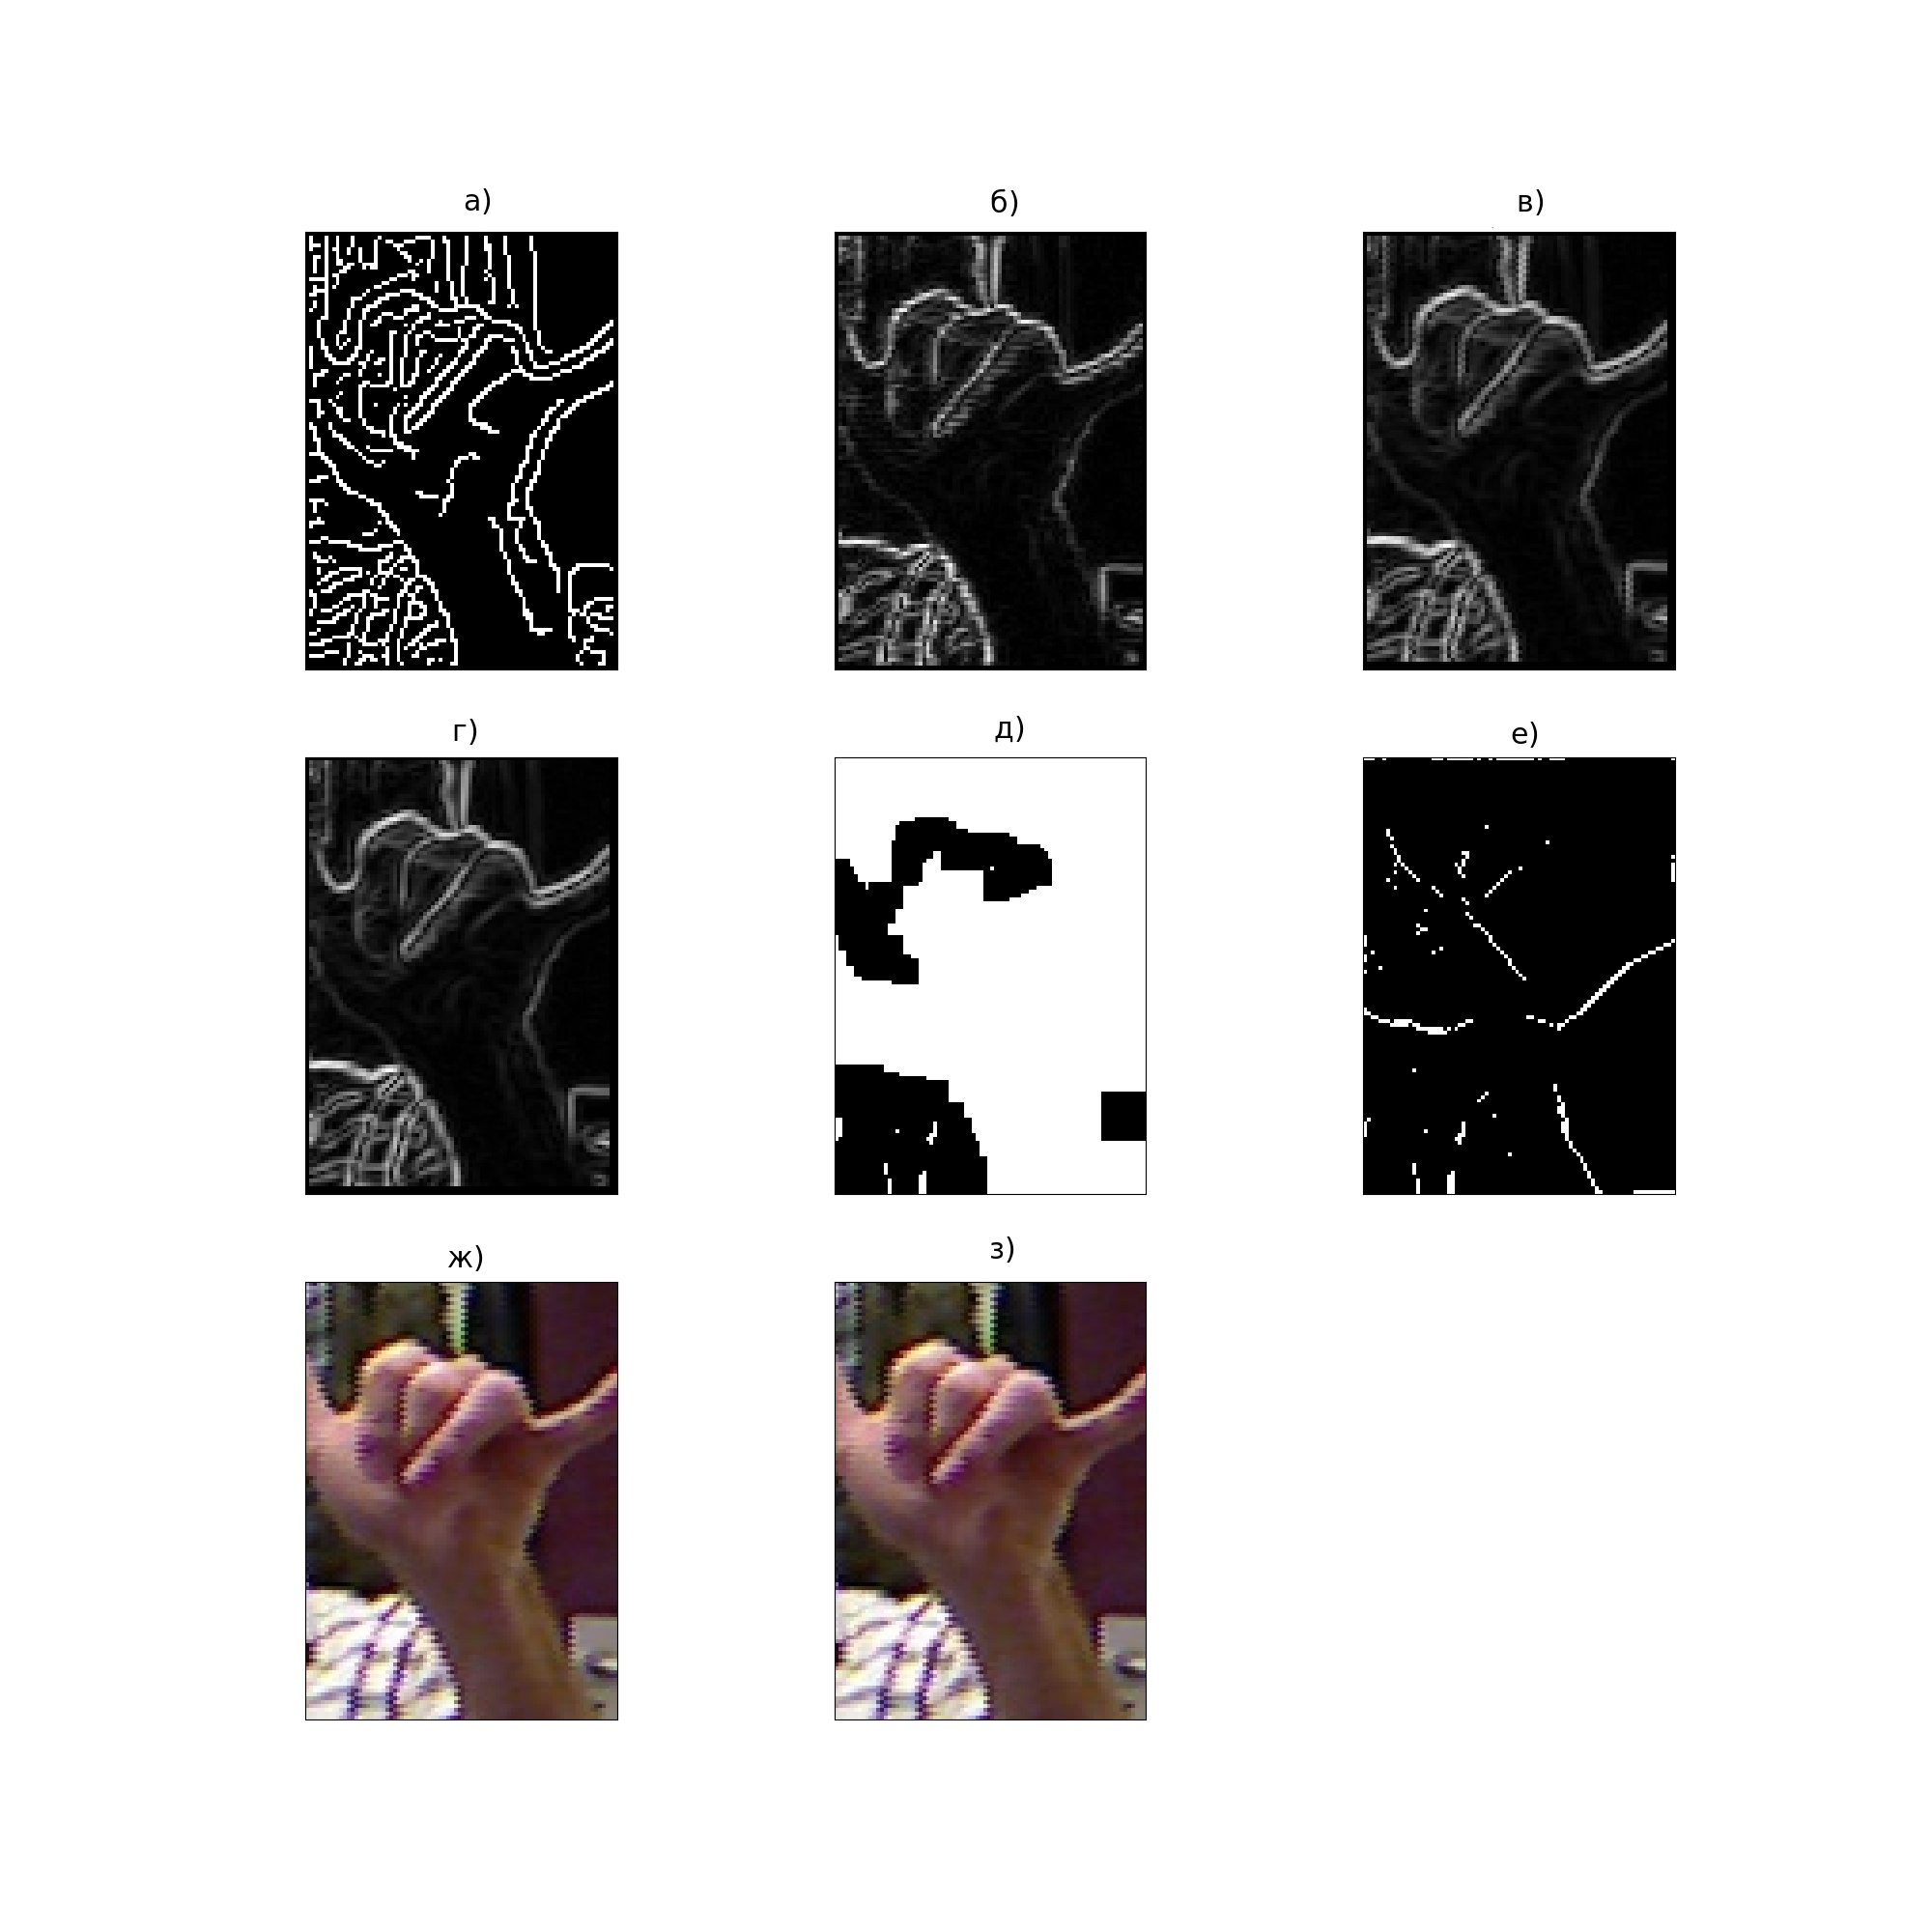
\includegraphics[width=\textwidth]{inc/img/compare1}
	\caption{Результат работы алгоритмов на наборе данных ASL Fingerspelling Images: а) оператор Кэнни; б) оператор Робертса; в) оператор Прюитт; г) оператор Собеля; д) выделение силуэта; е) морфологическое построение скелета; ж) построение скелета по ключевым точкам; з) оригинальное изображение}
	\label{an:compare}
\end{figure}

Морфологическое построение скелета показало время работы, сопоставимое с результатами оператора Кэнни (см. табл. \ref{tab:colombian-alphaber}, \ref{tab:asl2-alphaber}, \ref{tab:datamix-alphaber}). Итоговые результаты обработки изображения данным алгоритмом показали неудовлетворительное качество. Как говорилось выше, в результате получаются побочные ветви, а также скелет получается неполносвязным. В силу данных недостатков практически нецелесообразно использование данного алгоритма в построении метода классификации жестовых символов в силу зашумленности итоговых данных.

Алгоритм построения скелета по ключевым точкам не справился со своей задачей на большинстве изображениях, как видно на рис. 8. Однако, как показано на рис. \ref{an:compare2}, в случае успешного определения ключевых точек алгоритм безупречно производит построение скелетной модели жеста. Также для любого типа данных он работает за одно и то же время. В одних случаях это является преимуществом (табл. \ref{tab:colombian-alphaber}), в других — недостатком (табл. \ref{tab:asl2-alphaber}).

\begin{figure}[!h]
	\centering
	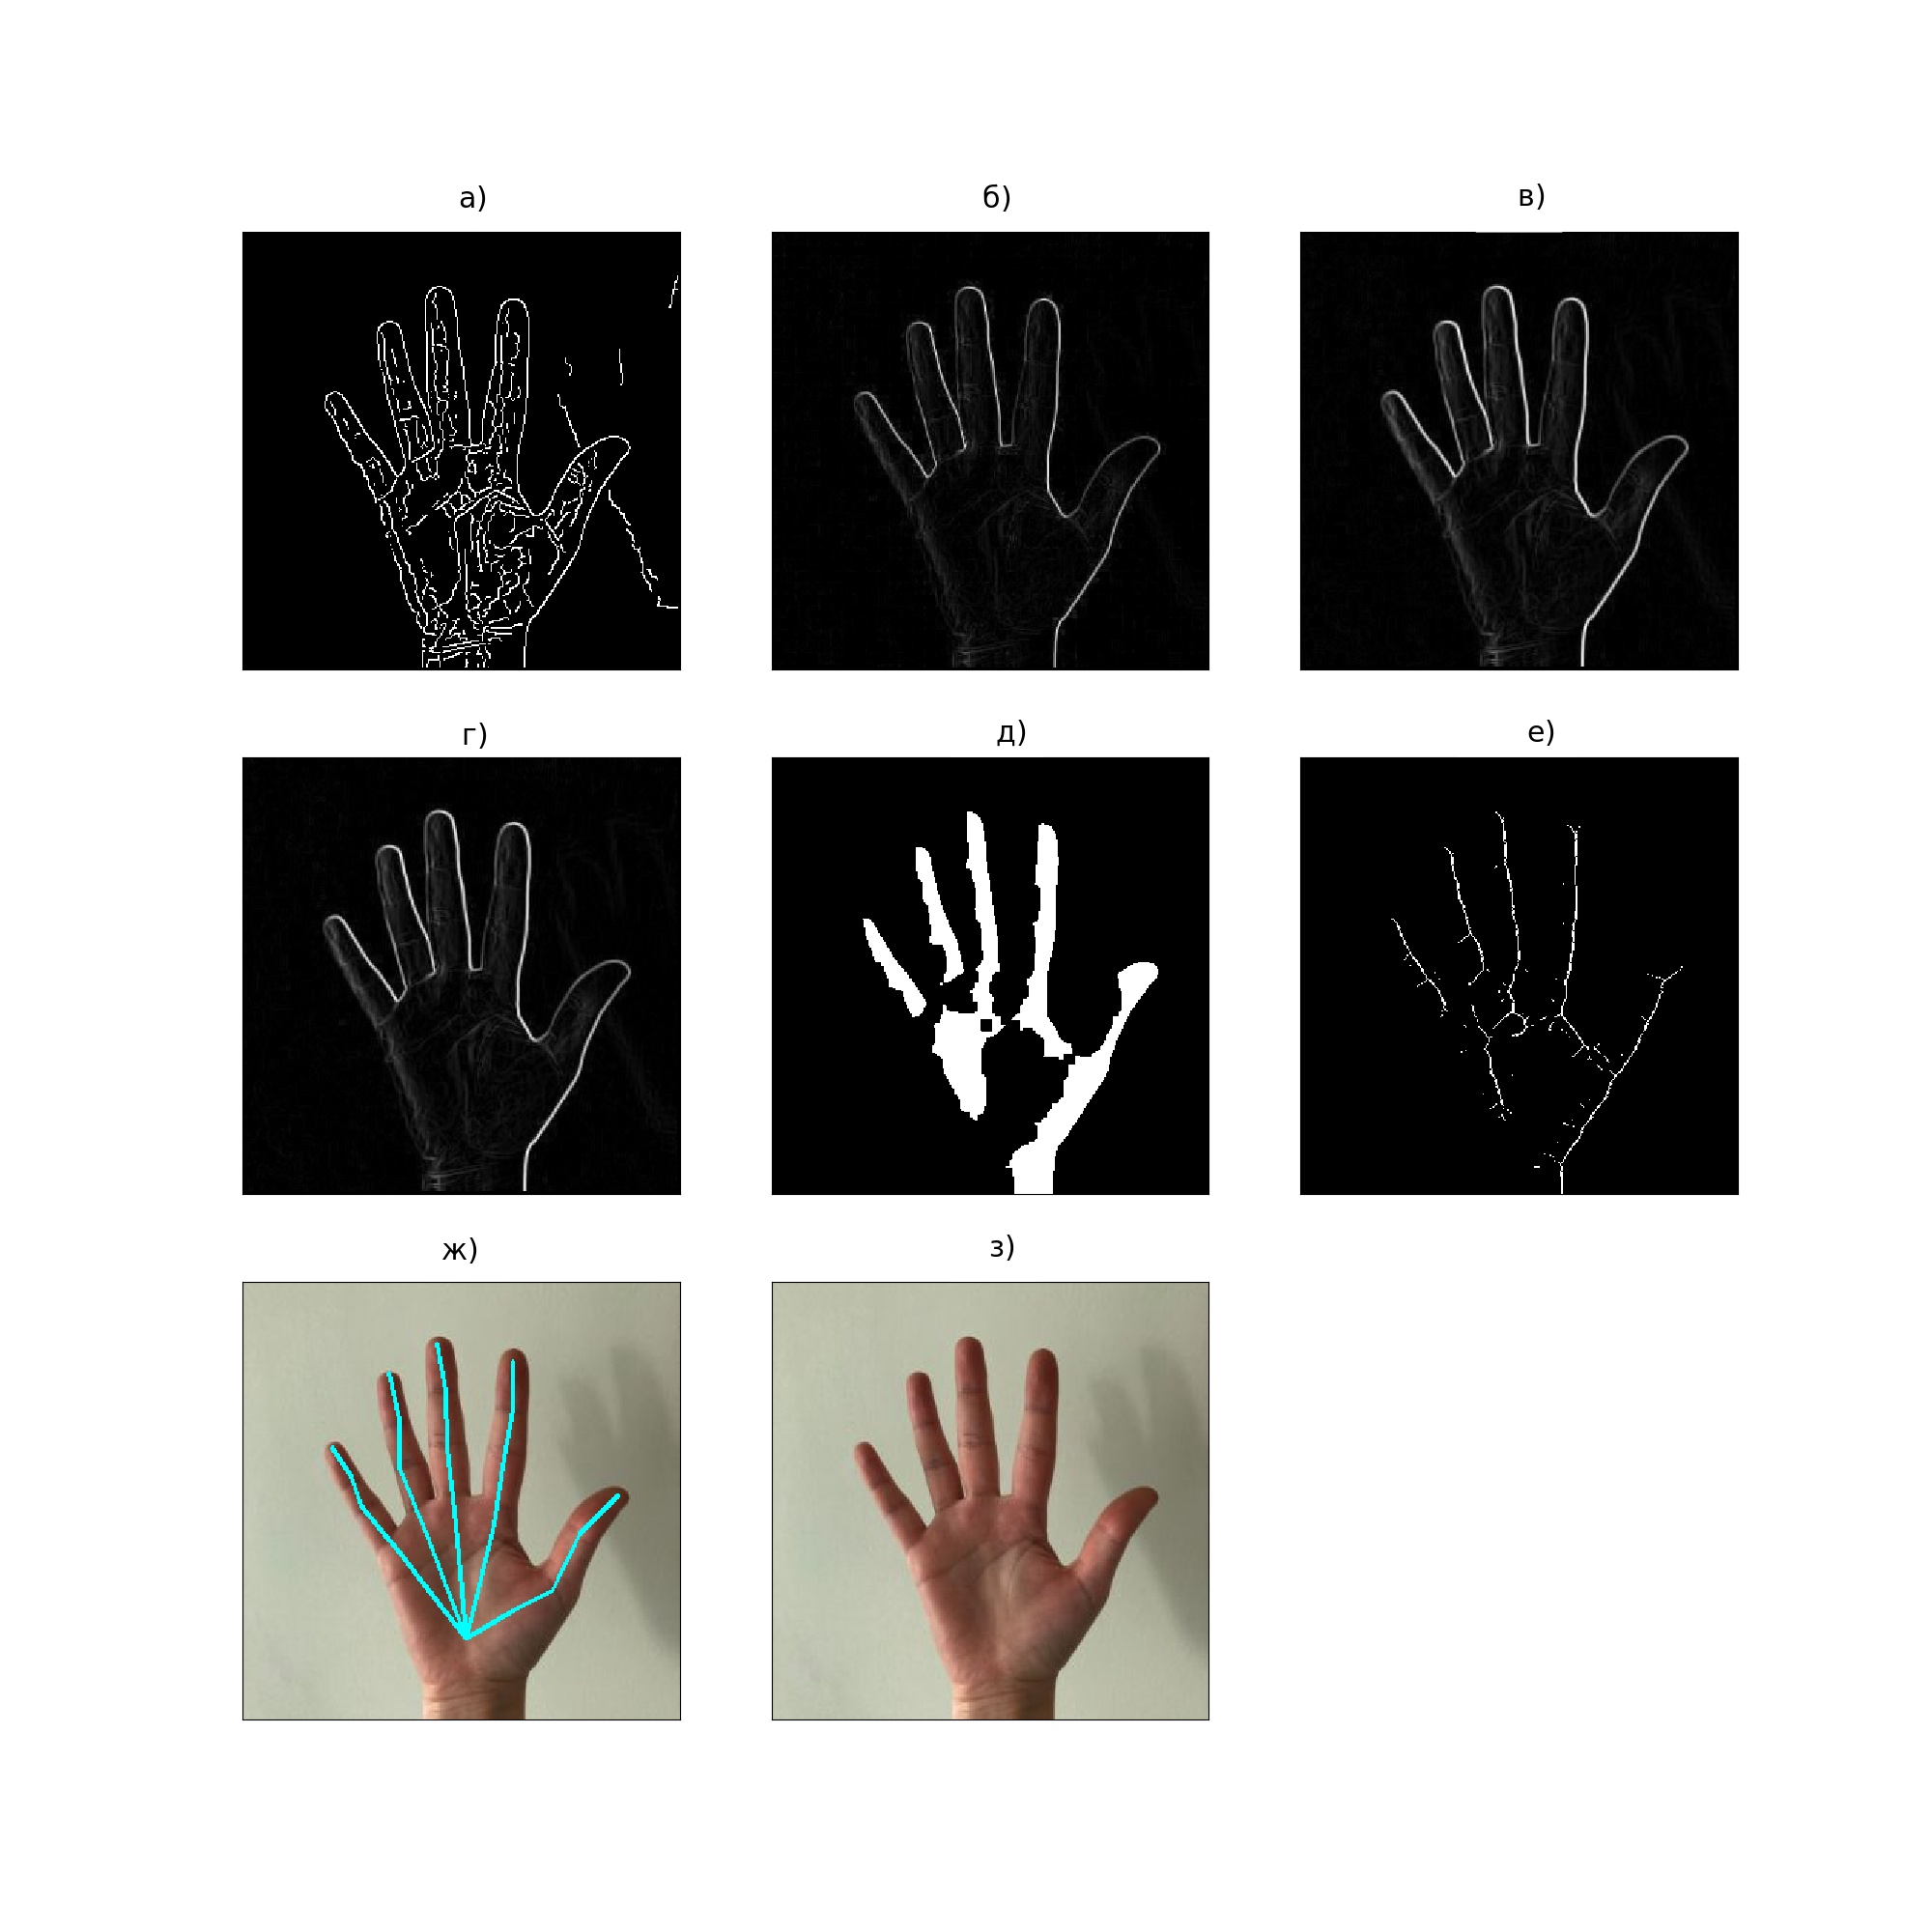
\includegraphics[width=\textwidth]{inc/img/compare2}
	\caption{Результат работы алгоритмов на наборе данных <<sign language between 0 9>>: а) оператор Кэнни; б) оператор Робертса; в) оператор Прюитт; г) оператор Собеля; д) выделение силуэта; е) морфологическое построение скелета; ж) построение скелета по ключевым точкам; з) оригинальное изображение}
	\label{an:compare2}
\end{figure}

\subsection{Вывод}

В результате проведенного сравнительного анализа были определены два метода. 

Выделение силуэта. Данный метод показал наименьшее время работы. Кроме того, бинарное изображение руки содержит в себе необходимые признаки жеста для его обработки классификатором.

Построение скелета по ключевым точкам. Скелетная модель является наилучшим типом входных данных для классификатора, т. к. не несет в себе никаких лишних данных\cite{Gil}.

Первый метод показал наилучшие результаты по скорости работы алгоритма,
кроме тестов на широкоформатных изображениях. В неудачных случаях (рис. \ref{an:compare}) второй метод не смог построить скелетную модель из-за неопределенных ключевых точек жеста.

\section{Методы классификации}

На данный момент известны следующие методы классификации жестовых символов:

\begin{itemize}
	\item скрытая марковская модель\cite{Zhang,Kasprzak};
	\item самоорганизующаяся карта Кохонена\cite{Tewari2012AVR,Karn,Starner};
	\item сверточные нейронные сети\cite{Potkin,10.1007/978-3-319-16178-5_40}.
\end{itemize}

\subsection{Скрытая марковская модель}

Одним из методов классификации, широкораспространенный в области распознавания жестов, является скрытая марковская модель (СММ). На ее основе построены системы распознавания китайского\cite{Zhang}, английского\cite{Starner} и польского\cite{Kasprzak} жестовых языков.

Скрытая марковская модель -- модель процесса, считающегося Марковским. Система представляет собой марковскую цепь, которая имеет конечное множество скрытых состояний, т.е. заданный момент времени неизвестно, в каком состоянии $s_i$ находится система. Каждое состояние $s_i$ может с некоторой вероятностью $b_{io_j}$ произвести событие $o_j$, которое можно наблюдать.

СММ $\lambda$ задается как $\lambda = \{S, \Omega, \Pi, A, B\}$, где $S=\{s_1, ..., s_n\}$ -- множество состояний, $\Omega = \{\omega_1, ..., \omega_m\}$ -- множество возможных событий, $\Pi = \{\pi_1, ..., \pi_n\}$ -- множество начальных вероятностей, $A = \{a_{ij}\}$ -- матрица вероятностей перехода из состояния $s_i$ в состояние $s_j$, $B = \{b_{i\omega_k}\}$ -- множество вероятностей наблюдения события $\omega_k$ после перехода системы в состояние $s_i$.

Задачи, решаемые с помощью СММ можно разделить на следующие группы:

\begin{itemize}
	\item кластерный анализ\cite{Helske} -- упорядочивание объектов в сравнительно однородные группы;
	\item регрессионный анализ\cite{Fridman} -- статистический метод исследования влияния одной или нескольких независимых переменных $x_1, ..., x_n$ на зависимую переменную $y$;
	\item задача классификации\cite{Benyacoub} -- разделение множества объектов некоторым образом на классы.
\end{itemize}

Задачу классификации можно трактовать как поиск вероятности попадания в состояние $s_n$ на шаге $t$. Для этого применяется алгоритм прямого-обратного хода. Обучение модели, происходящее с помощью алгоритма Витерби, заключается в подборе последовательности состояний, при которой вероятность заданной последовательности наблюдений является наибольшей. Алгоритм Баума-Велша меняет коэффициенты матрицы вероятности, максимизируя вероятность наблюдения последовательности событий $O$.

\subsection{Самоорганизующаяся карта Кохонена}

Самоорганизующиеся карты Кохонена(СКК) являются одной из разновидностей искусственных нейронных сетей. В области распознавания жестов нейросети данного типа могут применяться как для предобработки входных данных с целью извлечения признаков для классификатора\cite{Gao}, так и для распознавания самих жестов, например индийского\cite{Tewari2012AVR} и американского\cite{Karn} жестовых языков.

Основным отличием СКК от большинства известных нейронных сетей является обучение без учителя. При данном подходе процесс обучения не требует вмешательства со стороны и по этому результат будет зависеть только от структуры входных данных. Функцией СКК является кластеризация, то есть нет необходимости заранее знать классы выходных данных из обучающей выборки.

Архитектура сети состоит из двух слоев: входного и выходного, при этом каждый нейрон входного слоя связан с каждым нейроном выходного. Нейроны выходного слоя упорядочены и имеют структуру сетки. При этом каждый нейрон представляет собой n-мертный вектор вида $w=[w_1, ..., w_n]^T$, где $n$ равен размерности исходного пространства.

Процесс обучения разделяют на четыре основных этапа:

\begin{enumerate}
	\item Инициализация. Первоначальные веса узлов задаются случайными числами.
	\item Конкуренция. Нейроны вычисляют значения своей функции активации для каждого входного паттерна. Нейрон с наименьшим значением объявляется победителем.
	\item Объединение. Активный нейрон определяет пространственное расположение топологической окрестности нейронов, которые будут участвовать в процессе обучения. Размер окрестности определяется радиусом обучения.
	\item Подстройка весов. Выбранные нейроны уменьшают значения своих функций активации путем регулировки соответствующих весов узлов.
\end{enumerate}

Модификация весовых коэффициентов происходит по формуле \ref{eq:som-weights}.

\begin{eqnarray}\label{eq:som-weights}
w_i(t+1) = w_i(t) + h(t)*[x(t)-w(t)],
\end{eqnarray}

где
\begin{itemize}
	\item $t$ -- номер эпохи;
	\item $x(t)$ -- некоторый вектор из обучающей выборки;
	\item $h(t)$ -- функция соседства нейронов.
\end{itemize}

\subsection{Сверточные нейронные сети}

Создание сверточных нейронных сетей(СНС) было вдохновлено зрительной корой головного мозга человека\cite{Hubel}. Основное использование -- обработка изображений. Отличительной особенностью данной сети, подарившей ей название, является первый скрытый слой, работа которого похожа на процесс свертки двумерного изображения. В связи с этим, для большей наглядности входной слой вместо одномерного слоя нейронов можно рассматривать как двумерную матрицу, как в случае с файлом изображения. Для изображений значения этой двумерной матрицы представляют интенсивности пикселей. 

Рассмотрим особенности данной сети: сверточный и субдискретизирующий слои.

\section*{Слой свертки}

В отличии от обычной нейронной сети, в которой каждый нейрон входного слоя связан с каждым нейроном первого скрытого слоя, в СНС каждый нейрон в скрытом слое, называемом сверточным, связан только с нейронами, находящимися в определенной небольшой области (рис. \ref{anal:CNN-first}), которая определяется ядром свертки. Для формирования скрытого слоя ядро перемещается построчно по всей входной области, и может происходить с различным шагом, например на рисунке \ref{anal:CNN-first} шаг смещения равен 1.

\begin{figure}[!h]
	\centering
	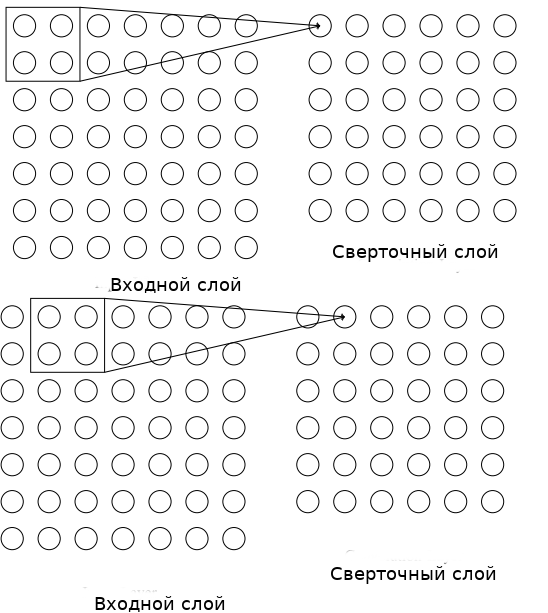
\includegraphics[width=0.55\textwidth]{inc/img/cnn-first.png}
	\caption{Связывание входного слоя с первым скрытым слоем}
	\label{anal:CNN-first}
\end{figure}

Размерность сверточного слоя определяется формулой \ref{eq:cnn-size}.

\begin{eqnarray}\label{eq:cnn-size}
(((W - X) / s) + 1) \times ((H - Y) / s) + 1), 
\end{eqnarray}

где

\begin{itemize}
	\item $W \times H$ -- размерность входного слоя;
	\item $X \times Y$ -- размерность ядра свертки;
	\item $s$ -- шаг смещения.
\end{itemize}

Результат нейрона $j,k$ сверточного слоя описывается формулой \ref{eq:cnn-result}.

\begin{equation}\label{eq:cnn-result}
a_{j,k} = \sigma \Bigg(b + \sum_{l=0}^{A-1} \sum_{m=0}^{B-1} w_{i,m}x_{j+l,k+m}\Bigg)
\end{equation}

Другими словами, сверточный слой выполняет функцию поиска первичных признаков входных данных, например границ изображения.

\section*{Слой субдискретизации}

Слой субдискретизации (англ. Pooling) выполняет задачу уменьшения размерности данных через нелинейное уплотнение. Исходная область разбивается на области, к которым, независимо друг от друга, происходит уплотнение области до одного значения. Пример работы данного слоя предоставлен на рисунке \ref{anal:CNN-pooling}.

\begin{figure}[!h]
	\centering
	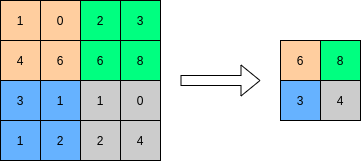
\includegraphics[width=0.6\textwidth]{inc/img/pooling}
	\caption{Cубдискретизация с функцией максимума и фильтром 2$\times$2 с шагом 2}
	\label{anal:CNN-pooling}
\end{figure}

Размер области задается фильтром, который обычно равен $2 \times 2$. В качестве функции фильтра обычно используют функцию максимума. Но так же применимы и другие, например функции среднего значения и L2-нормирования. 

Другими словами работу слоя субдискретизации можно описать следующим образом: если при работе сверточного слоя уже были выявлены некоторые признаки, то в дальнейшем настолько подробные данные уже не нужны, то есть можно их сократить до менее подробных.

\section*{Общая архитектура СНС}

В задачах распознавания жестовых символов СНС уже применялась для работы с русским\cite{Potkin} и итальянским\cite{10.1007/978-3-319-16178-5_40} жестовыми языками. Не смотря на разницу в архитектурных особенностях методов, общий подход к построению сети можно разделить на следующие слои:

\begin{enumerate}
	\item Сверточный слой.
	\item Слой субдискретизации.
	\item Полносвязный слой.
\end{enumerate}

\subsection{Сравнительный анализ выделенных методов классификации}

В результате анализа предметной области были рассмотрены три метода классификации жестовых символов. Каждый класс обладает рядом функциональных преимуществ, которые выделяют его на фоне других подходов. В то же время имеется и ряд недостатков, который ограничивает область применимости данно­го класса методов.

Сравнение преимуществ и недостатков рассмотренных решений представлено в таблице \ref{anal:longtable-classificators}.

\begin{center}
	\begin{longtable}{|p{0.30\textwidth}|p{0.32\textwidth}|p{0.32\textwidth}|}
		\caption{Сравнительный анализ методов классификации}
		\label{anal:longtable-classificators}
		\\ \hline
		Название метода & Преимущества & Недостатки \\
		\hline \endfirsthead
		\subcaption{Продолжение таблицы~\ref{anal:longtable-classificators}}
		\\ \hline \endhead
		\hline \subcaption{Продолжение на след. стр.}
		\endfoot
		\hline \endlastfoot
		СММ & Простая математическая структура & Каждая модель обучается только на экземплярах своего класса \\
		& Возможность использования исходных данных без предобработки & Большое число неструктурированных параметров \\
		&& Максимизация отклика модели на свои классы без минимизации на другие \\
		\hline
		Самоорганизующаяся карта Кохонена & Обучение без учителя & Окончательный результат зависит от начальных установок \\
		& Устойчивость к зашумленным данным &\\
		& Скорость обучения &\\
		\hline
		СНС & Частичная инвариантность к масштабу & Склонность к переобучению \\
		& Частичная инвариантность к повороту и сдвигу & Необходимость в большой обучающей выборке \\
		& Созданы специально для обработки изображений &  \\
	\end{longtable}
\end{center}

Сравнительный анализ качества классификации на американском жестовом языке выделенных методов представлено в таблице \ref{anal:longtable-accuracy}.

\begin{center}
	\begin{longtable}{|p{0.60\textwidth}|c|}
		\caption{Точность работы методов классификации}
		\label{anal:longtable-accuracy}
		\\ \hline
		Название метода & Точность \\
		\hline \endfirsthead
		\subcaption{Продолжение таблицы~\ref{anal:longtable-accuracy}}
		\\ \hline \endhead
		\hline \subcaption{Продолжение на след. стр.}
		\endfoot
		\hline \endlastfoot
		СММ\cite{Starner} & 90,7 -- 93,5\%  \\
		\hline
		Самоорганизующаяся карта Кохонена\cite{Karn}& 92\% \\
		\hline
		СНС\cite{Garcia} & 97,82\% \\
	\end{longtable}
\end{center}

Как видно из таблицы, использование СНС дает наилучший результат классификации в задачах распознавания жестовых символов. Данный тип нейронной сети изначально рассчитан на обработку изображений. 

\subsection{Капсульные нейронные сети}

Капсульные нейронные сети (англ Capsule Neural Network) -- предназначенная для распознавания изображений архитектура нейронных сетей. КНС были задуманы Джеффри Хинтоном в 1979 году, первые работы по ней опубликованы в 2017 году\cite{sabour2017dynamic}. Идея данной сети является следствием критики сверточных нейронных сетей. Полученная в ходе свертки информация о входных данных частично теряется на этапе субдискретизации. Например в задачи распознавания лиц данная сеть учитывает наличие на изображении глаз, ушей, носа и губ, но игнорирует их взаимное расположение. Следствием этого может быть ложное распознавание деформированного лица, пример которого представлен на рисунке \ref{anal:CNN-bad}.

\begin{figure}[!h]
	\centering
	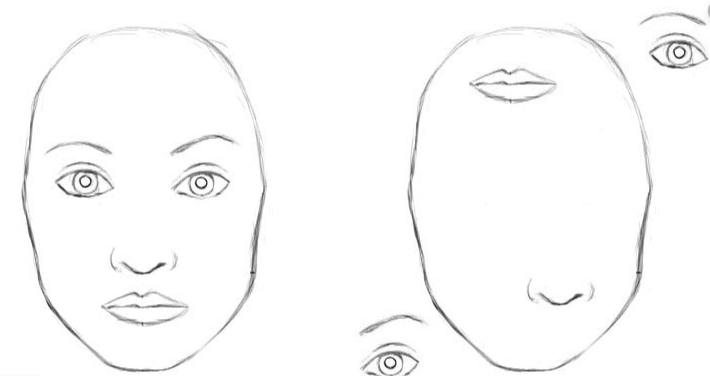
\includegraphics[width=0.6\textwidth]{inc/img/face_deformed}
	\caption{Деформированное изображение лица}
	\label{anal:CNN-bad}
\end{figure}

Особенностью КНС являются капсулы -- группа нейронов, инкапсулирующая информацию о состоянии функции, которую обнаруживают в векторной форме. 

В отличии от обычных нейронов, работающих со скалярными величинами, капсулы работают с векторами. Вычисление выходного значения капсулы происходит в соответствии с формулой \ref{eq:caps-sum}, представляющее собой скалярное произведение векторов.

\begin{eqnarray}\label{eq:caps-sum}
s_j = \sum_{i}c_{ij}\hat{u}_{i|j} \quad	\hat{u}_{i|j} = W_{ij}u_i,
\end{eqnarray}

где

\begin{itemize}
	\item $u_i$ -- вектор входных значений;
	\item $W_{ij}$ -- матрица аффинного преобразования;
	\item $c_{ij}$ -- коэффициент маршрутизации;
	\item $s_j$ -- выходное значение.
\end{itemize}

Заменой функции активизации, применяемой в нейронах для задания нелинейности данным, в капсулах является нормализация нормализация выходного вектора по формуле \ref{eq:caps-norm}.


\begin{eqnarray}\label{eq:caps-norm}
v_j = \frac{{||s_j||}^2}{1 + {||s_j||}^2} \frac{s_j}{||s_j||}
\end{eqnarray}

Итоговые различия между капсулами и обычными нейронами представлена в таблице \ref{tab:caps2trad}.

\begin{table}[!h]
	\caption{\label{tab:caps2trad}Различия между капсулами и нейронами}
	\begin{center}
		\begin{tabular}{|c|c|c|}
			\hline
			Параметр & Капсула & Нейрон \\
			\hline
			Формат входных данных & вектор $(u_i)$ & скаляр $(x_i)$ \\
			\hline
			Преобразование входных данных & $\hat{u}_{i|j} = W_{ij}u_i$ & -- \\
			\hline
			Сумматор & $s_j = \sum_{i}c_{ij}\hat{u}_{i|j}$ & $a_j = \sum_{i}w_ix_i + b$ \\
			\hline
			Передаточная функция & $v_j=\frac{{||s_j||}^2}{1 + {||s_j||}^2}\frac{s_j}{||s_j||}$ & $h_j=f(a_j)$ \\
			\hline
			Формат выходных значений & вектор $(v_j)$ & скаляр $(h_j)$ \\
			\hline
		\end{tabular}
	\end{center}
\end{table}

Капсулы являются расширением нейронов до векторной формы, что позволяет хранить, обрабатывать и передавать больше информации. Например в задачах распознавания лиц капсула может хранить не только признаки присутствия глаза на изображении, но и дополнительную информацию о его положении относительно других частей.

Благодаря этим особенностям данная архитектура инвариантна к поворотам и смещениям изображения, обучение происходит быстрее и требует меньший объем выборки. Применение данной архитектуры позволяет сократить ошибку классификации при поворотах на 43\%, в сравнении с СНС\cite{em}. Эти утверждения были экспериментально доказаны на датасете рукописных цифр MNIST\cite{sabour2017dynamic}.

Автор предлагает использование КНС в качестве классификатора при построении метода классификации жестовых символов.

\section{Вывод}

Были представлены этапы работы известных методов распознавания жестовых символов. Рассмотрены возможные способы получения информации, их преимущества и недостатки. 

Проведен сравнительный анализ методов предобработки изображений. Показано преимущество выделения силуэта кисти руки в сравнении с остальными методами с точки зрения скорости и качества выделения признаков с изображения.

Сравнительный анализ методов классификации показал, что СНС имеет наилучшее качество распознавания среди рассмотренных классификаторов. Принято решение использование данного решения в качестве базового при построении метода распознавания жестовых символов. Не смотря на высокую точность классификации, СНС имеют проблемы с инвариантностью к пространственным изменениям изображения, а также требуют большого объема обучающей выборки. В качестве альтернативы предложено использование КНС, архитектура которых направлена на устранение описанных недостатков сверточных сетей.